% the abstract
\chapter*{Foreword}
\phantomsection
\addcontentsline{toc}{chapter}{Foreword}
\setlength\parindent{0pt}
\vspace{-1cm}
The big red button. In every bioinformatics-oriented presentation my supervisor gave over the years of my PhD studentship this familiar slide reappeared.
It is the biologist's dream; a mythical and mystical red button that takes their raw data and transforms it magically into a \emph{Nature} paper ready for submission.


Of course this is an unattainable dream, but there are many steps we can take to easy the burden of data analysis and decrease the
turnaround time between sample collection and manuscript submission.

\begin{center}
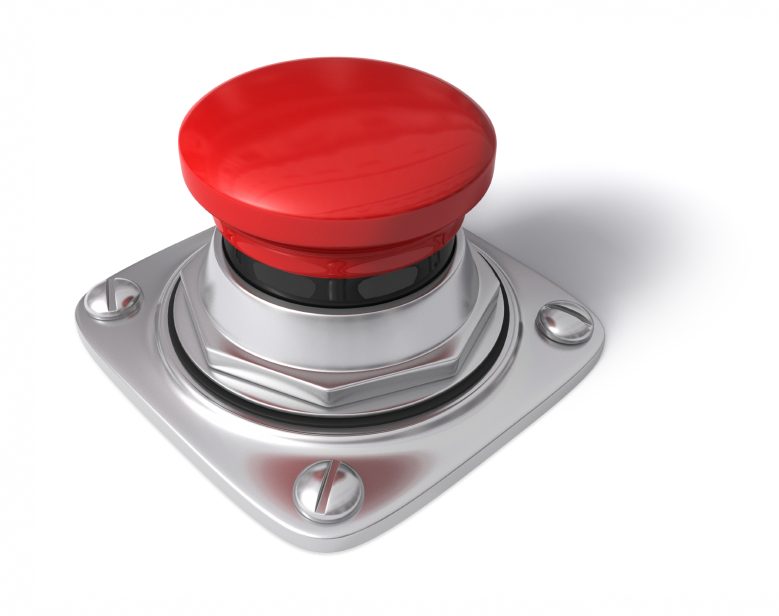
\includegraphics[scale=0.25]{chapters/images/redbutton.jpg}
\end{center}
